\documentclass[10pt,conference,compsocconf]{IEEEtran}

\usepackage[utf8]{inputenc}
%\usepackage{times}
%\usepackage{balance}
\usepackage[breaklinks]{hyperref}
\usepackage{graphicx}	% For figure environment
\usepackage{amsmath}
\usepackage{amssymb}
\usepackage{amsfonts}
\usepackage{subfigure}

\begin{document}
\title{Inpainting by Sensitive Mean Filtering}

\author{
  Leo Büttiker \mbox{    }  Urs Fässler \mbox{     } Nicolas Rüegg \\
  Group moebs, Department of Computer Science, ETH Zurich, Switzerland

}

\maketitle

\begin{abstract}
  A task often required in image processing is inpainting -- the reconstruction of missing pixels where the location of the missing pixels is known. While many different methods for inpainting exist, we present a particularly intuitive method based on \emph{Mean Filtering}. Our method called \emph{Inpainting by Sensitive Mean Filtering} is extremly fast and achieves qualitatively good results. To support this claim we present results of our method compared to \emph{Inpainting with Overcomplete Dictionaries} and an algorithm based on partial differential equations.
\end{abstract}


%%%%%%%%%%%%%%%%%%%%%
\section{Introduction}
Images often contain missing values for certain pixels or pixel patches. Examples are scratches or random noise in an image.
Using an inpainting method, one tries to approximate values for these pixels. In \emph{Inpainting with Overcomplete Dictionaries}, overcomplete Haar wavelet or DCT dictionaries are often used to reconstruct the missing pixels. These methods both proved to be quite slow even for relatively small images. Another algorithm for inpainting is \emph{Inpainting NaNs} -- an algorithm based on partial differential equations.

In this paper, we present a simpler and faster method for inpainting of small parts of images. In section \ref{sec:mean_filtering}, we describe our \emph{Inpainting by Sensitive Mean Filtering} method. It is an intuitive and simple method in which missing pixel values are approximated by using existing neighboring pixels.

Experiments discussed in \ref{sec:results} have shown that considering random noise, our method achieves appealing results over a broad range of images.

In section \ref{sec:discussion} we discuss the advantages and disadvantages in terms of computation time and error of our method in comparison to the methods \emph{Inpainting with Overcomplete Dictionaries} and \emph{Inpainting NaNs}.

Finally, section \ref{sec:future} gives an outlook on future work and section \ref{sec:summary} summarizes our results.


%%%%%%%%%%%%%%%%%%%%%
\section{Sensitive Mean Filtering}
\label{sec:mean_filtering}
The \emph{Sensitive Mean Filter} is an extension of the well known \emph{mean filter} as described in \cite{McDonnell198165}. This algorithm sets the value of every pixel to the mean of itself and its surrounding pixels. This is based on the idea that values of spatial close pixels usually just vary moderately.

Unlike the classical \emph{mean filter}, our method uses a bitmask which indicates the missing pixels. By exploiting this additional information, we can build the mean just over given pixels and can also guarantee not to corrupt correct pixels.

Our method can formally be described as follows:
Let $f_{m,n}$ be a $[0,1]$ pixel value of a $M \times N$ gray scale image and let $l$ be the given $M \times N$ mask indicating the missing pixels, where
\begin{equation}
 l_{m,n} = 
 \left\{
 \begin{array}{ll}
  1 & \text{if pixel (m,n) is set} \\
  0 & \text{if pixel (m,n) missing}
 \end{array}
 \right.
\end{equation}

For a $(2K + 1) \times (2L + 1)$ kernel, we calculate the value of a pixel $f'_{i,j}$ in the approximation of the image $f'$ as follows:
\begin{equation}
\label{eqn:sensitivMean}
 f'_{i,j} = 
  \frac{\sum\limits_{m=i-K}^{i+K}\sum\limits_{n=j-L}^{j+L} f_{m,n}}{\sum\limits_{m=i-K}^{i+K}\sum\limits_{n=j-L}^{j+L} l_{m,n}} 
\end{equation}
We assume missing pixels in $f$ to be set to 0. Therefore, formula \ref{eqn:sensitivMean} calculates the mean over the given correct pixels.

We calculate the value for $f'_{i,j}$ on a $3 \times 3$ kernel as long as the denominator is not equal to zero. I.e., a pixel is surrounded by at least one given pixel. If this approach fails, we take a  $5 \times 5$ kernel. If this also fails, we set the missing pixel to the overall mean of the image.

As a post processing step, smoothing is performed. For this we use the Linear Noise Cleaning method as described in \cite{Pratt1991}. 

In a first step, we set the given correct pixels from $f$ in the approximated image $f'$ and apply a discrete convolution on it with the impulse response array $H_1$. It defines a low-pass noise cleaning filter.

\begin{equation}
H_1 =
  \frac{1}{100}
  \begin{bmatrix} 1 & 8 & 1\\ 8 & 64 & 8 \\ 1 & 8 & 1 \end{bmatrix}
\end{equation}

In a second step, we set the given correct pixels from $f$ again and use a different filter $H_2$. This kernel places emphasis on the directly neighboring pixels.

\begin{equation}
H_2 =
  \frac{1}{8}
  \begin{bmatrix} 0 & 1 & 0\\ 1 & 4 & 1 \\ 0 & 1 & 0 \end{bmatrix}
\end{equation}

As a final step, we set the given correct pixels from $f$ for the last time to get the reconstructed image.

\emph{Sensitive Mean Filtering} can be implemented computationally efficient as a set of matrix operations.

%%%%%%%%%%%%%%%%%%%%%
\section{Results}
\label{sec:results}
From a subjective point of view, our method achieves visually excellent results for missing patches of less than $5 \times 5$ pixels. This is true for randomly as well as non-randomly missing pixels as Figure \ref{fig:lena_results} and Figure \ref{fig:pepper_results} show.

\begin{figure*}[ht]
\centering
\subfigure[Original]{
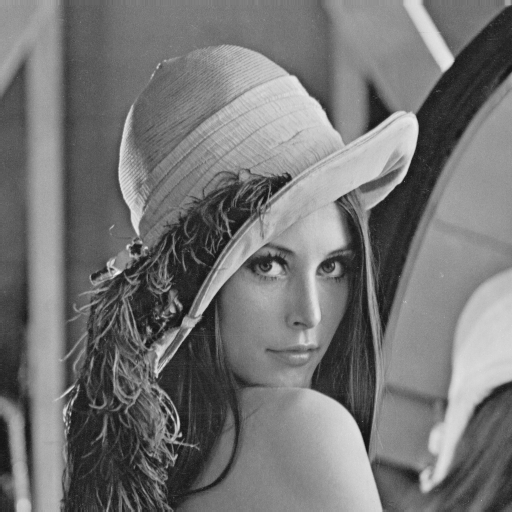
\includegraphics[width=0.31\linewidth]{images/lena_original.png}
\label{fig:lena_original}
}
\subfigure[With missing pixels]{
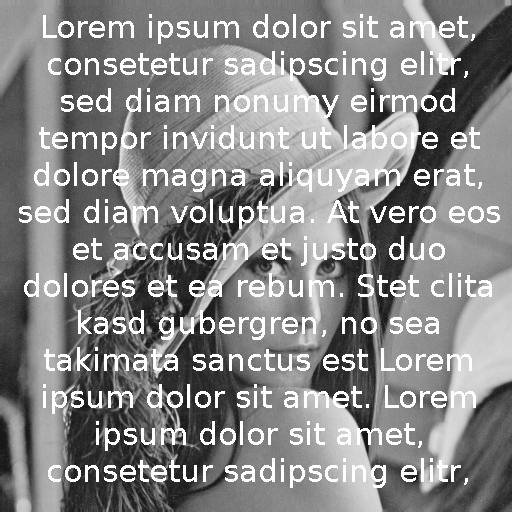
\includegraphics[width=0.31\linewidth]{images/lena_destroyed.png}
\label{fig:lena_destroyed}
}
\subfigure[Reconstructed with Sensitive Mean Filtering]{
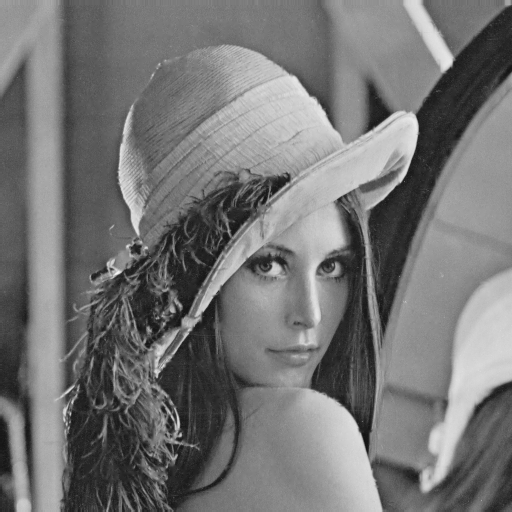
\includegraphics[width=0.31\linewidth]{images/lena_sensitiv.png}
\label{fig:lena_reconstructed}
}
\caption[]{The \emph{Inpainting by Sensitive Mean Filtering} Method achieves visually appealing results on relatively small non-randomly missing pixels.\label{fig:lena_results}}
\end{figure*}


\begin{figure*}[ht]
\centering
\subfigure[Original]{
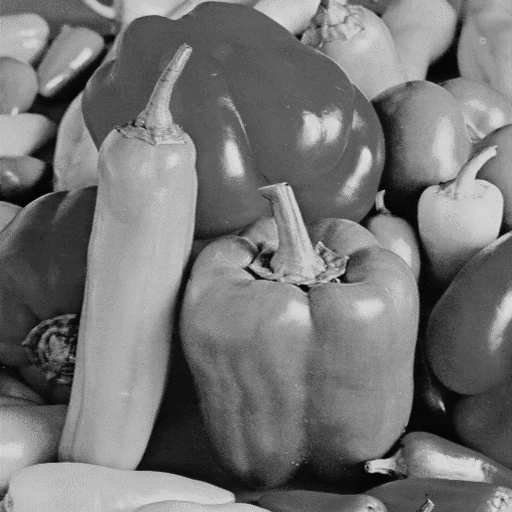
\includegraphics[width=0.31\linewidth]{images/peppers_original.png}
\label{fig:peppers_original}
}
\subfigure[With $80\%$ missing pixels]{
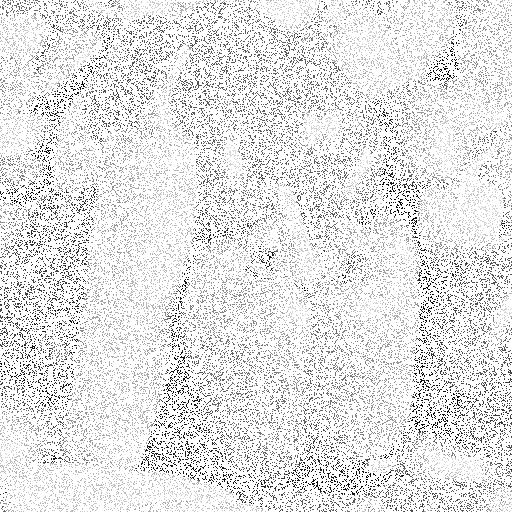
\includegraphics[width=0.31\linewidth]{images/peppers_80_error.png}
\label{fig:peppers_destroyed}
}
\subfigure[Reconstructed with Sensitive Mean Filtering]{
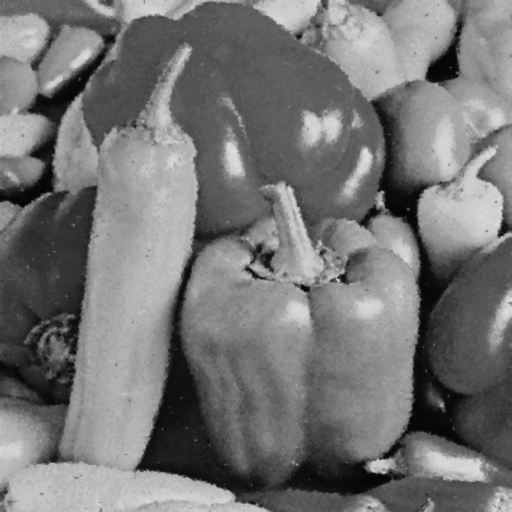
\includegraphics[width=0.31\linewidth]{images/peppers_80_sensitiv.png}
\label{fig:peppers_reconstructed}
}
\caption[]{The \emph{Inpainting by Sensitive Mean Filtering} Method achieves visually appealing results on relatively small patches of randomly missing pixels.\label{fig:pepper_results}}
\end{figure*}

We tested our method on twelve different $512 \times 512$ gray scale images, each with ten different masks of missing pixels. Each mask consisted of $60\%$ randomly missing pixels. The set of images encompasses the categories \emph{Natural Pictures}, \emph{Comics} and \emph{Textures} with four images in each one. The category \emph{Natural Pictures} includes photographs, \emph{Comics} contains comic images with hard transitions of intensity and \emph{Textures} consists of photographs of small repeating structures such as a brick wall or grass.

To quantify the error of our method, we used the Mean Square Error (MSE) over every single reconstructed image:

\begin{equation}
\label{eqn:mse}
\mathit{MSE} = \frac{1}{M\,N}\sum_{i=1}^{M}\sum_{j=1}^{N} [f_{i,j} - f'_{i,j}]^2
\end{equation}


The visually appealing result in Figures \ref{fig:lena_results} and \ref{fig:pepper_results} is confirmed by the expectation value over all MSEs which is 0.0054. The standard deviation is 0.0076.

The experiments also showed that our method does not depend on the mask for randomly generated masks.

Figure \ref{fig:error_vs_category} shows that our method achieves significantly smaller errors on the category  \emph{Natural Pictures} than on the category \emph{Comics} and \emph{Textures}, respectively. The expectation value of the error on \emph{Natural Pictures} is 0.0011. For \emph{Comics} it is at 0.0093 and for \emph{Textures} at 0.0057. We assume this to be due to the harder transitions of intensity in \emph{Comics} and fine-grained structures in \emph{Textures}.
%Stddev : 0.00072549439862, 0.01080922130026, 0.0050570999883

\begin{figure}[ht]
\centering
 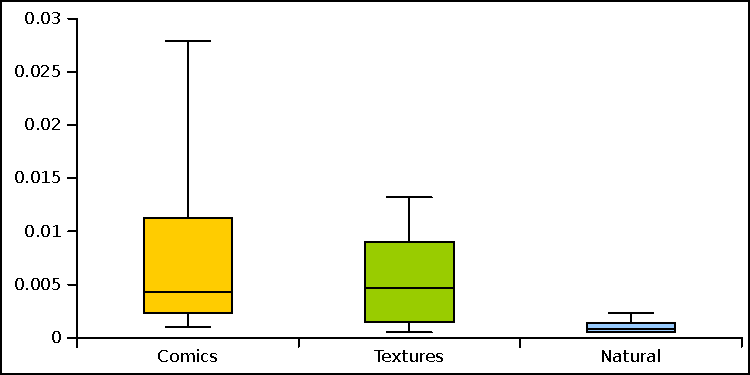
\includegraphics[width = \linewidth]{images/errorDependingOnCategorie.pdf}
\caption[]{Error (MSE) depending on the image category. Generated on the test set of the twelve images and ten randomly generated masks of $60\%$ missing pixels.\label{fig:error_vs_category}}
\end{figure}

On $512 \times 512$ images, our method implemented in \emph{Matlab} running on an Intel Core i5 CPU M 520 at 2.40GHz with 4GB memory needs approximately $0.26$ seconds. It does not depend on the rate of of missing pixels as Figure \ref{fig:time_vs_missing_pixels} shows.


%%%%%%%%%%%%%%%%%%%%%
\section{Discussion}
\label{sec:discussion}
In this section we look at our method's advantages and disadvantages and compare it to \emph{Inpainting with Overcomplete Dictionaries} with a Haar wavelet dictionary and a DCT dictionary, as well as to \emph{Inpainting NaNs}.

\emph{Inpainting NaNs} is a boundary value solver. It is described by its author as follows\cite{john06}: ''The basic idea is to formulate a partial differential equation (PDE) that is assumed to apply in the domain of the artifact to be inpainted. The perimeter of the hole supplies boundary values for the PDE. Then the PDE is approximated using finite difference methods (the array elements are assumed to be equally spaced in each dimension) and then a large (and very sparse) linear system of equations is solved for the NaN elements in the array.'' In our context, the NaN elements are the missing pixels.
%
%The method use a basically elliptic PDE. This means that the resulting linear system will generally be well conditioned.
%
%Neat hah? For an arbitrary number of NaN elements in an array, the above scheme is all there is to method 2 of inpaint\_nans, together with a very slick application of sparse linear algebra in Matlab.''


\emph{Inpainting with Overcomplete Dictionaries} is implemented as described in \cite{buhman11}. The parameters for the Haar wavelet and DCT dictionary are chosen as in \cite{aharon06}. I.e., the image is split into non-overlapping patches of size $8 \times 8$ and the individual patches are coded into vectors $x \in \mathbb{R}^{64}$. With the vectorized pixel patches as columns, the entire image is coded in a matrix $X \in \mathbb{R}^{64 \times (d/8)^2}$, where $d$ is the side length of the quadratic image in pixels. For DCT as well as Haar wavelets, the dictionary  $U \in \mathbb{R}^{64 \times 441}$ contains 441 linearly dependent atoms.  Finally, using a \emph{Matching Pursuit} algorithm, matrix $X$ is approximated by atoms from the overcomplete dictionary $U$.\footnote{The algorithm to generate the overcomplete Haar wavelet dictionary was taken from \cite{christen10}. The algorithm to generate the overcomplete DCT dictionary was taken from \cite{rubinstein09}, \cite{rubinstein09soft}.}

An experiment over the test set of the twelve images and ten randomly generated masks of $60\%$ missing pixels confirmed the competitiveness of our method. The resulting error is shown in Figure \ref{fig:error_vs_algorithm}. As Figure \ref{fig:error_vs_missing_pixels} shows, \emph{Inpainting by Sensitive Mean Filtering} also performs good for lower and higher rates of missing pixels than $60\%$.

\begin{figure}[ht]
\centering
 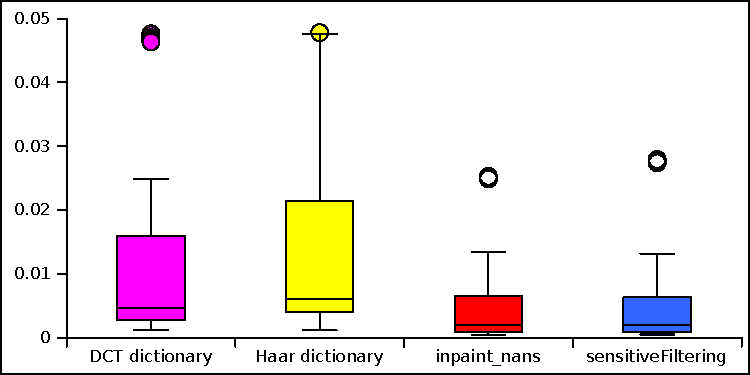
\includegraphics[width = \linewidth]{images/errorDependingOnAlgorithm.pdf}
\caption[]{Error (MSE) depending on the inpainting method. Generated on the test set of twelve images and ten randomly generated masks of $60\%$ missing pixels.\label{fig:error_vs_algorithm}}
\end{figure}

\begin{figure}[ht]
\centering
 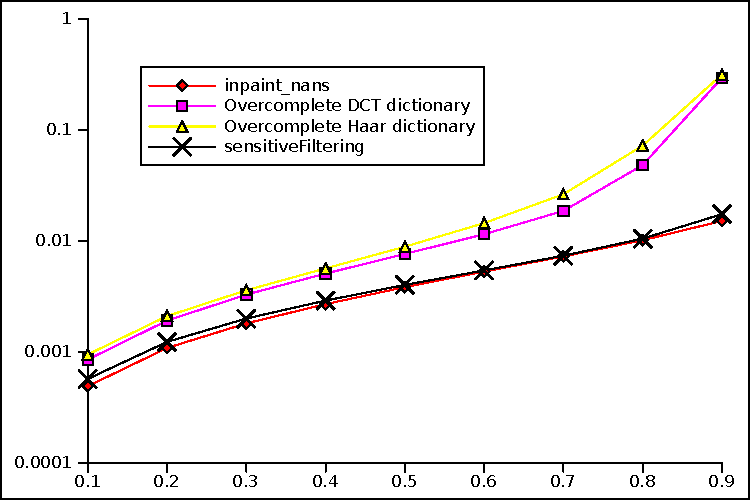
\includegraphics[width = \linewidth]{images/errorDependingOnMissingPixels.pdf}
\caption[]{Error (MSE) depending on the rate of missing pixels. Generated on the test set of twelve images and ten randomly generated masks of missing pixels for every rate of missing pixels.\label{fig:error_vs_missing_pixels}}
\end{figure}

But despite of the fact that \emph{Inpainting by Sensitive Mean Filtering} achieves competitive results regarding the quality of the result, its biggest advantage is its speed. On the test set of twelve different images and ten different masks of randomly missing pixels ($60\%$ missing), our method is significantly faster than the other methods as is shown in Figure \ref{fig:time_vs_method}. % Additionally, Figure \ref{fig:time_vs_missing_pixels} shows that unlike \emph{Inpainting NaNs}, the running time of our method is almost independent of the rate of missing pixels.

\begin{figure}[ht]
\centering
 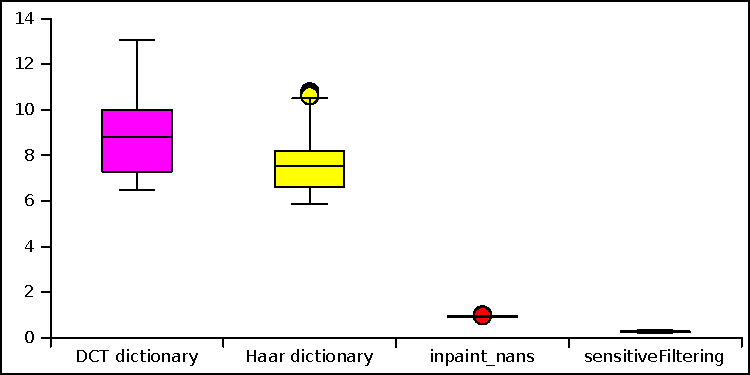
\includegraphics[width = \linewidth]{images/timeDependingOnAlgorithm.pdf}
\caption[]{Time in seconds depending on the inpainting method. Generated on the test set of twelve images and ten randomly generated masks of $60\%$ missing pixels. The means are 9.1 (DCT dictionary), 7.7 (Haar dictionary), 0.93 (inpaint\_nans) and 0.26 (sensitiveFiltering) seconds.\label{fig:time_vs_method}} 
\end{figure}


\begin{figure}[ht]
\centering
 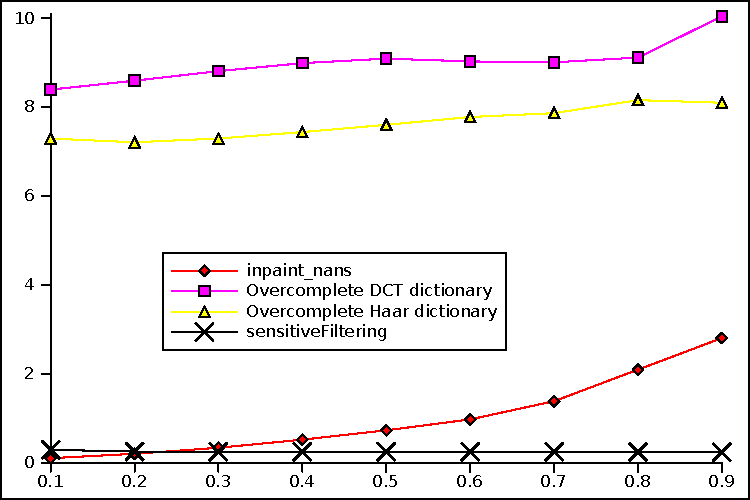
\includegraphics[width = \linewidth]{images/timeDependingOnMissingPixels.pdf}
\caption[]{Time in seconds depending on rate of missing pixels. Generated on the test set of twelve images and ten randomly generated masks of missing pixels for every rate of missing pixels.\label{fig:time_vs_missing_pixels}}
\end{figure}

Despite all its advantages, one has to consider that our method is not well suited for missing pixel patches of more than $5 \times 5$ pixels as experiments with larger patches of missing pixels have shown. This is due to our method's dependence on spatial close pixels and the relatively small choice of the kernel, which for the implementation described in this paper is of size $5 \times 5$ maximally.


%%%%%%%%%%%%%%%%%%%%%
\section{Future Work}
\label{sec:future}
To overcome the dependence on relatively small patches of missing pixels, we also developed a method called \emph{Inpainting by Clustering}. It is based on the idea that within an image, there exist many similar areas. In this method, an image is divided into (possibly overlapping) pixel patches of equal size which then are vectorized. Subsequently, these vectors are grouped into clusters using \emph{k-means}. The actual inpainting is done by setting the missing pixels of a vector to the corresponding pixel values of the assigned cluster's centroid.

A set of non-scientifically conducted experiments lets us assume that this method also achieves good results regarding the error, but can by no means compete with the presented \emph{Inpainting by Sensitive Mean Filtering} in terms of speed. Nevertheless, for applications with large patches of missing pixels where computing power is not an issue, further investigation of the \emph{Inpainting by Clustering} method might be worthy.

Considering the presented method \emph{Inpainting by Sensitive Mean Filtering}, it could be interesting to investigate in what extent an iterative version could improve the results for missing pixel patches of large scale. Furthermore it should be investigated if border detection could help to improve the algorithm on images with hard transitions, e.g. our  \emph{Comics} test set. Especially for masks with large missing patches, an algorithm with an adaptive kernel size might also be worth to consider.


%%%%%%%%%%%%%%%%%%%%%
\section{Summary}
\label{sec:summary}
The experiments for small patches of missing pixels (less than $5 \times 5$) have shown, that our method \emph{Inpainting by Sensitive Mean Filtering} is superior to the methods \emph{Inpainting with Overcomplete Dictionaries} and \emph{Inpainting NaNs} in terms of speed, with no losses in quality.
Due to the relatively fast computation time, our method is in particular an eligible candidate for applications with high demands on speed or little computing power.

Our method also shows that for small areas of missing pixels, a simple algorithm can achieve very good results.

\bibliographystyle{IEEEtran}
\bibliography{report}
\end{document}
